\PassOptionsToPackage{hyphens}{url}
\documentclass[final,5p,twocolumn,a4paper]{elsarticle}

\usepackage{amssymb}
\usepackage{amsmath}
\usepackage{hyperref}
\usepackage{graphicx}
\usepackage{booktabs}
\usepackage{listings}
\usepackage{xcolor}
\usepackage{float}
\usepackage{url}
\usepackage{enumitem}
\setlist{noitemsep, topsep=2pt, parsep=0pt, partopsep=0pt, leftmargin=1.4em}

\setlength{\textfloatsep}{5pt plus 2pt minus 2pt}
\setlength{\intextsep}{5pt plus 2pt minus 2pt}
\setlength{\dbltextfloatsep}{5pt plus 2pt minus 2pt}
\setlength{\floatsep}{5pt plus 2pt minus 2pt}
\setlength{\dblfloatsep}{5pt plus 2pt minus 2pt}
\setlength{\abovedisplayskip}{4pt plus 2pt minus 2pt}
\setlength{\belowdisplayskip}{4pt plus 2pt minus 2pt}

\definecolor{codegreen}{rgb}{0,0.6,0}
\definecolor{codegray}{rgb}{0.5,0.5,0.5}
\definecolor{codepurple}{rgb}{0.58,0,0.82}
\definecolor{backcolour}{rgb}{0.96,0.96,0.96}
\lstdefinestyle{mystyle}{backgroundcolor=\color{backcolour}, commentstyle=\color{codegreen},
    keywordstyle=\color{blue}, numberstyle=\tiny\color{codegray}, stringstyle=\color{codepurple},
    basicstyle=\ttfamily\scriptsize, breaklines=true, captionpos=b, keepspaces=true, numbers=left,
    numbersep=5pt, showspaces=false, showstringspaces=false, showtabs=false, tabsize=2}
\lstset{style=mystyle}

\journal{SoftwareX}

\begin{document}

\begin{frontmatter}

\title{LunarAtlas: A Reproducible Data Processing and Interactive Visualization Infrastructure for Chandrayaan-3 LIBS Level-1 Archives}

\author[MDU]{Lovekesh Anand\corref{cor1}}
\ead{lovekeshanand6@gmail.com}
\author[MDU]{Dua Saeed (duasaeed641@gmail.com)}
\address[MDU]{Department of Computer Science and Engineering, Maharshi Dayanand University, Rohtak, Haryana, India}
\cortext[cor1]{Corresponding author}

\begin{abstract}
LunarAtlas is open-source software that turns the publicly archived Chandrayaan-3 laser-induced breakdown spectroscopy (LIBS) Level-1 (L1) products into relational, query-ready, L1-derived spectral records. The L1 tables store 2,094 wavelength channels as columns and interleave plasma and background acquisitions. LunarAtlas parses the PDS4 labels, verifies each data file against the checksum declared in its label, reshapes the tables, pairs every plasma acquisition with the most recent preceding background acquisition, subtracts and clamps, records pairing and clipping provenance, and serves the result through a REST API and a web viewer. On the full local copy of the calibrated archive (301 products, 1,281 acquisitions) all 1,582 data files matched their label checksums, all products parsed, 613 of 745 plasma acquisitions were paired and 132 without a preceding background were excluded; repeated processing produced byte-identical spectral outputs and repeated database ingestion added no rows. An LTTB-based downsampler optionally preserves caller-specified channels; preserving the detected peaks of a worked-example spectrum costs 9--22~a.u.\ of RMSE at an equal 130-point budget. Wavelength-coincidence annotation against a 24-line reference list is provided for exploration only; it is not elemental identification, and archive-wide coincidences were not statistically significantly enriched under the specified random-shift null ($p\approx0.10$).
\end{abstract}

\begin{keyword}
LIBS \sep Chandrayaan-3 \sep planetary spectroscopy \sep PDS4 \sep relational database \sep downsampling \sep REST API
\end{keyword}
\end{frontmatter}

\section*{Required Metadata}

\begin{table*}[!ht]
\centering
\small
\begin{tabular}{|l|p{7.5cm}|p{7.5cm}|}
\hline
\textbf{Nr.} & \textbf{Code metadata description} & \textbf{Please fill in this column} \\
\hline
C1 & Current code version & v1.0.1 (archived); revised code on branch \texttt{revision/audit-v2} (new archived release pending) \\
\hline
C2 & Permanent GitHub link to code/repository used for this code version & \href{https://github.com/LovekeshAnand/LunarAtlas}{https://github.com/LovekeshAnand/LunarAtlas} \\
\hline
C3 & Legal Code License & MIT License \\
\hline
C4 & Code versioning system used & git \\
\hline
C5 & Software code languages, tools, and services used & Python 3.11, SQL, TypeScript, HTML, CSS \\
\hline
C6 & Compilation requirements, operating environments \& dependencies & Python~3.11, PostgreSQL (16.3 local in the original benchmarks, 18 in the revision checks; 15.x remote Supabase), Node.js~18.x, Redis (optional cache); numpy, pandas, scipy, fastapi, React \\
\hline
C7 & If available Link to developer documentation/manual & \href{https://github.com/LovekeshAnand/LunarAtlas}{https://github.com/LovekeshAnand/LunarAtlas} \\
\hline
C8 & Support email for questions & lovekeshanand6@gmail.com \newline duasaeed641@gmail.com \\
\hline
\end{tabular}
\caption{Code metadata (mandatory)}
\label{table:metadata}
\end{table*}

\section{Motivation and Significance}

Laser-Induced Breakdown Spectroscopy (LIBS) is an established technique for in-situ elemental analysis in planetary exploration, deployed on ChemCam \cite{maurice2012chemcam, wiens2012chemcam}, SuperCam \cite{maurice2021supercam, wiens2021supercam} and MarSCoDe \cite{xu2021marscode}. In 2023 the LIBS payload on the Chandrayaan-3 Pragyan rover acquired the first in-situ LIBS spectra from the lunar south polar region \cite{megala2024chandrayaan, sridhar2024libs, isro_chandrayaan3_libs}.

The instrument uses a pulsed 1535~nm laser and a flat-field grating spectrometer with a linear CCD; its stated calibrated range is 220--800~nm \cite{sridhar2025libs}. The L1 parent tables carry 2,094 channels labelled 164.35--878.26~nm, spaced $\approx$0.34~nm. This spacing is a sampling interval, not a resolution; the stated optical resolution, below 1.1~nm FWHM \cite{sridhar2025libs}, is treated as an upper bound, so lines closer than this may be unresolved. Data are distributed by the ISRO PRADAN portal as PDS4 products \cite{isro_chandrayaan3_libs, pds4_standard}.

The L1 products are preserved but not query-ready: (i) all 2,094 channels are columns, complicating relational storage and range queries; (ii) plasma and background acquisitions are interleaved and must be distinguished by status flags; (iii) analysis of plasma emission usually starts from background-subtracted spectra; and (iv) interactive viewing of many 2,094-channel spectra benefits from downsampling.

To our knowledge, no documented open-source workflow covers these steps for this archive. Table~\ref{table:capability_comparison} compares LunarAtlas with \emph{pds4\_tools} \cite{pds4_tools_ref} and \emph{libpyhat} \cite{anderson2019libpyhat}. \emph{pds4\_tools} reads the label and table but does not interpret the wavelength columns or acquisition flags; \emph{libpyhat} provides preprocessing and multivariate workflows on spectra that are already in its MultiIndex layout. LunarAtlas covers the step between PDS4 delivery and such toolkits. It does not perform elemental identification or abundance retrieval.

\begin{table*}[!htbp]
\centering
\small
\begin{tabular}{lccc}
\toprule
\textbf{Capability} & \textbf{pds4\_tools} \cite{pds4_tools_ref} & \textbf{libpyhat} \cite{anderson2019libpyhat} & \textbf{LunarAtlas} \\
\midrule
PDS4 XML label parsing & Yes & No & Yes \\
Label-checksum verification of data files & No & No & Yes \\
Wavelength-column axis reconstruction & No & No & Yes \\
Plasma/background flag parsing ($F$, $L$) & No & No & Yes \\
Measured-background subtraction with pairing provenance & No & No & Yes \\
Wide-to-long relational reshaping & No & No & Yes \\
Spectral preprocessing (norm, baseline, PCA) & No & Yes & Partial$^\dagger$ \\
Relational database ingestion, REST API, web viewer & No & No & Yes \\
Elemental identification / abundance retrieval & No & Partial & No \\
\bottomrule
\multicolumn{4}{p{0.95\textwidth}}{\footnotesize $^\dagger$ ALS and Savitzky--Golay smoothing are optional, display-only API filters; normalisation/PCA/ML remain the domain of tools such as libpyhat, with which LunarAtlas CSV output is compatible.}
\end{tabular}
\caption{Capability comparison (LunarAtlas revision branch).}
\label{table:capability_comparison}
\end{table*}

\section{Software description}

\subsection{Software Architecture}

LunarAtlas has three tiers (Figure~\ref{fig:architecture}). PostgreSQL \cite{postgresql} stores product and file metadata, raw acquisitions and background-subtracted plasma acquisitions in long form, together with pairing and clipping fields. A Python~3.11/FastAPI service \cite{fastapi} serves them with an optional Redis cache \cite{redis}, optional display-only ALS/Savitzky--Golay filters, and server-side LTTB downsampling when a request sets \texttt{zoom\_level} or \texttt{proportion}. The two kinds of client process data differently: the React \cite{react} web viewer requests full-resolution spectra and downsamples them in the browser (TypeScript, Web Worker), whereas scripts and other API clients receive server-downsampled or full-resolution JSON. Developer endpoints under \texttt{/api/v1/public} require an API key; the viewer endpoint \texttt{/api/v1/spectrum} (Listing~\ref{lst:api}) is not authenticated.

\begin{figure*}[t]
    \centering
    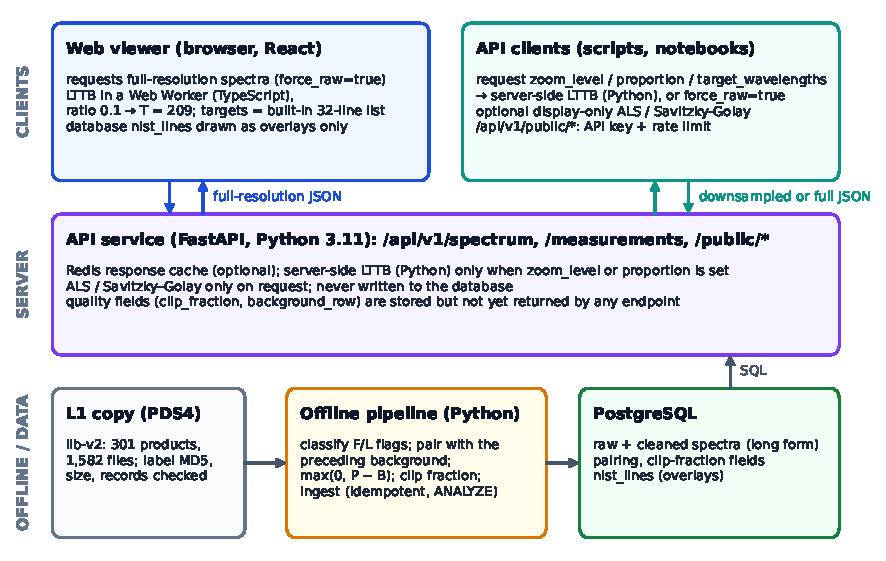
\includegraphics[width=0.8\textwidth]{../figures/fig1_architecture}
    \caption{System architecture. Server-side Python LTTB runs only when a request sets \texttt{zoom\_level} or \texttt{proportion}; the web viewer fetches full-resolution spectra and downsamples them in the browser (TypeScript), whereas API clients receive server-downsampled or full-resolution JSON.}
    \label{fig:architecture}
\end{figure*}

\subsection{Data processing pipeline}
\label{subsec:pipeline}

The pipeline is a sequence of scripts (inventory, L1 processing, QA plots, checksum manifest, database ingestion, audit). L1 processing performs:

\begin{enumerate}
    \item \textbf{Label parsing and integrity check.} Logical identifier, times and file attributes are read from each PDS4 label \cite{pds4_standard}. The MD5 checksum, size and record count declared in the label are compared with the data file (Section~\ref{subsec:archive}). This establishes file integrity, not the correctness of later processing.
    \item \textbf{Wide-to-long reshaping} of the 2,094 channel columns into $(\text{measurement},\lambda)\rightarrow I$ after checking the eight trailing instrument-parameter columns.
    \item \textbf{Acquisition classification} from the Force-Reset ($F$) and Laser-Fire ($L$) flags: background $B$: $(F{=}1,L{=}0)$; plasma $P$: $(F{=}0,L{=}1)$; $(0,0)$, $(1,1)$ and missing flags are logged and skipped. The same rule is used for raw and cleaned records in the database, so a global identifier \texttt{\{file\_info\_id\}-\{n\}} names the same $n$-th plasma acquisition in both tables.
    \item \textbf{Pairing.} Each plasma acquisition is paired with the most recent preceding background acquisition in file order; consecutive plasma acquisitions reuse it. Plasma acquisitions with no preceding background are excluded from the cleaned tables (their raw rows are ingested only when the same product also has paired acquisitions). The row of the paired background is stored with every cleaned acquisition.
    \item \textbf{Measured-frame subtraction and clamping:}
    \begin{equation}
        \label{eq:clamping}
        I_{\mathrm{clean}}(\lambda) = \max\bigl(0,\, I_{P}(\lambda) - I_{B}(\lambda)\bigr).
    \end{equation}
    This assumes that the background frame is additive and unchanged between the two acquisitions. Label timestamps have 1~s resolution, so the actual interval is known only to within a second (Section~\ref{subsec:archive}). Clamping removes negative residuals and therefore biases low-signal spectra upwards relative to the unclamped difference.
    \item \textbf{Clip fraction.} For each cleaned acquisition, the fraction of the 2,094 stored channels with $I_P - I_B < 0$ \emph{before} clamping is stored (\texttt{clip\_fraction}); channels where $I_P = I_B$ are not counted. Acquisitions above 0.5 receive a warning. The flag excludes nothing from storage.
\end{enumerate}

Measured-frame subtraction is distinct from the optional ALS \cite{eilers2003perfect} and Savitzky--Golay \cite{savitzky1964} filters, which are applied only to API responses on request and never written to the database.

\subsubsection{LTTB downsampling with preserved channels}
\label{subsec:lttb}

For zoom level $k$ the server computes a budget $T(k)=\min\!\bigl(2094,\ \lfloor 2094\cdot2^{-k}\rfloor\bigr)$ (alternatively $\lfloor 2094\,p\rfloor$ for a proportion $p$), independent of how many channels fall inside the requested wavelength window, and returns all points if $T$ is not smaller than that number. LTTB \cite{steinarsson2013lttb} partitions the window into $T-2$ index buckets and keeps, per bucket, the point that maximises the triangle area with the previously kept point and the mean of the next bucket. The caller may pass a list of target wavelengths; the channel nearest to each target (with no distance limit, so out-of-window targets map to an end channel) is added:
\begin{equation}
\begin{aligned}
S_{\mathrm{final}} &= S_{\mathrm{LTTB}}(T) \cup \{i^{*}(t) : t \in \mathcal{T}\},\\
i^{*}(t) &= \arg\min_i |\lambda_i - t|,\qquad |S_{\mathrm{final}}| \le T + |\mathcal{T}|.
\end{aligned}
\end{equation}
The algorithm does not detect peaks. The web viewer runs a TypeScript implementation of the same rule on all 2,094 channels with $T=209$ (ratio 0.1) and its built-in 32-line target list; the 33 database \texttt{nist\_lines} are display overlays only. In Section~\ref{subsec:ds} the detected peaks are passed as targets (``LTTB+Peaks''), so their retention is 100\% by construction. An equal-budget variant that fits LTTB+Peaks into $T$ points is an evaluation construct, not production code; its construction is given in Supplementary Section~S3.

\subsubsection{Candidate wavelength coincidences}
\label{subsec:nist}

Peaks are found with \texttt{scipy.signal.find\_peaks} in 220--800~nm with prominence $\ge 3\sigma$ ($\sigma$: population standard deviation of the cleaned spectrum over 560--580~nm) and $\ge5$ channels separation. A peak is a \emph{candidate coincidence} if at least one of 24 reference wavelengths (Fe, Mg, Si, Al, Ti, Ca, Na, H, O lines from the NIST ASD \cite{nist_asd}, listed in \texttt{Pipeline/step4\_nist\_verification\_logs.py}) lies within $|\lambda_{\mathrm{obs}}-\lambda_{\mathrm{ref}}|<0.5$~nm; each peak counts once regardless of how many references fall within the tolerance. A coincidence is not an identification: the list is short and incomplete (e.g.\ only one O~I 777~nm triplet component), several references lie within 1.1~nm of one another and may be unresolved, and the L1 wavelength scale itself is uncertain (Section~\ref{subsec:archive}).

\subsection{Testing}
\label{subsec:testing}

The \texttt{pytest} suite runs the real stage-2 processor on synthetic L1 files (pairing, exclusion of unpaired plasma, identifier stability, pre-clamp clip fraction, background provenance, ambiguous flags) and tests the server LTTB implementation; an ingestion test against a disposable PostgreSQL database checks identifier linkage, the quality fields and idempotent re-ingestion. Continuous integration runs the non-database tests for Python 3.10--3.12.

\section{Illustrative examples}

A demonstration deployment runs at \url{https://www.lunaratlas.in} with the API at \url{https://apis.lunaratlas.in}; the citable artifact is the archived code \cite{lunaratlas_zenodo}. Setup follows \texttt{pip install -r requirements.txt}, \texttt{npm install} and \texttt{./run\_pipeline.sh} as documented in the README. Listing~\ref{lst:api} requests a downsampled, smoothed spectrum from the public deployment, which still holds legacy-ingested records (Section~\ref{subsec:archive}). For this identifier, a paired acquisition in both versions, the unsmoothed response matched the revision output on all 2,094 channels when checked on 23 October 2026. The listing is \texttt{revision\_v2/api\_example.py}; \texttt{LUNARATLAS\_API} points it at another server.

\begin{lstlisting}[language=Python, caption=Python client request for a downsampled spectrum (public demonstration deployment), label=lst:api]
import requests
url = "https://apis.lunaratlas.in/api/v1/spectrum"
params = {"measurement_id": "FI-20230825-104221-00-3",
          "lambda_min": 240.0, "lambda_max": 450.0,
          "zoom_level": 2, "als": True, "savgol": True}
r = requests.get(url, params=params, timeout=30)
r.raise_for_status()
for pt in r.json()["data"][:5]:
    print(pt["wavelength_nm"], pt["intensity"])
\end{lstlisting}

\section{Impact and evaluation}

We separate four levels: (A) archive-wide ingestion validation, (B) detailed evaluation of spectral processing on one worked-example product, (C) candidate annotation, and (D) scientific identification or abundance analysis, which this work does not attempt. All numbers below are produced by the scripts and settings in \texttt{revision\_v2/} from one input version (Section~\ref{subsec:archive}).

\subsection{Archive-wide ingestion validation}
\label{subsec:archive}

The input is a local copy (\texttt{datasets/uploads}) of the PRADAN Chandrayaan-3 LIBS calibrated archive \texttt{lib-v2}: labels created 2024-05-16, nine mission days (25 August--2 September 2023), 301 products. The copy's original download date was not recorded and the original download location is no longer available; the label checksums below are therefore the evidence that the copy matches the archive's own description. Table~\ref{table:audit} reconciles all counts.

\begin{table}[!htbp]
\centering
\footnotesize
\setlength{\tabcolsep}{3pt}
\begin{tabular}{@{}p{5.4cm}r@{}}
\toprule
\textbf{Item} & \textbf{Count} \\
\midrule
Products discovered / parsed / failed & 301 / 301 / 0 \\
Data files (301 parent tables, 1,281 single-shot files) & 1,582 \\
\quad MD5 equal to label value$^{a}$ & 1,582 \\
\quad size equal to label value & 1,582 \\
Parent tables with 2,094 channels, identical axis & 301 \\
Acquisitions: background / plasma & 536 / 745 \\
\quad ambiguous or missing flags; NaN intensities & 0; 0 \\
Plasma paired / without preceding background & 613 / 132 \\
\quad paired with the immediately preceding row & 416 \\
Products: with paired plasma / background only / plasma, none with a preceding background$^{b}$ & 230 / 33 / 38 \\
Duplicate logical IDs; duplicate measurement IDs & 0; 0 \\
Cleaned points ($613\times2{,}094$) & 1,283,622 \\
\bottomrule
\multicolumn{2}{p{7.6cm}}{\scriptsize $^{a}$91 label checksums are printed without leading zeros (30 or 31 hex digits); all match after left-padding to 32 digits. $^{b}$Disjoint categories covering all 301 products; of the 38, 34 contain no background row and in 4 the only background follows the last plasma row (118 plasma rows in total).}
\end{tabular}
\caption{Archive audit of the 301-product L1 copy (\texttt{revision\_v2/audit\_archive.py}).}
\label{table:audit}
\end{table}

\textit{Earlier counts.} The 779 measurements reported previously came from an earlier processing version that also stored the 132 unpaired plasma acquisitions without subtraction and 34 background frames as cleaned records ($613+132+34=779$). The public deployment still holds these legacy records; a reversible migration has been rehearsed on a disposable copy but not applied (Supplementary Section~S1).

\textit{Pairing intervals.} With 1~s timestamp resolution, the paired background carries the same second as the plasma acquisition for 206 acquisitions, the previous second for 264 and 2--13~s earlier for 143, so the stable-background assumption spans up to 13~s for some pairs.

\textit{Archive wavelength scale.} Each acquisition is also archived as a single-shot table (Wavelength, Response count). Its counts are identical to the corresponding parent-table row in all 1,281 cases, but its wavelength column is a different axis (153.21--873.30~nm), offset from the parent-table axis by $-4.96$ to $-11.14$~nm ($-7.48$~nm at 589~nm). LunarAtlas uses the parent-table axis throughout. We cannot determine from the archive which axis is correct; this is consistent in magnitude with the L1 calibration offsets reported by Mourlin et al.\ \cite{mourlin2025chandrayaan} and directly limits wavelength-based annotation.

\textit{Determinism and ingestion.} Two stage-2 runs produced byte-identical spectral outputs for all 230 products. Ingestion into a disposable PostgreSQL~18 database stored 613 cleaned acquisitions (1,283,622 points) matching the files exactly, a second ingestion added no rows, and every stored cleaned value equals $\max(0,I_P-I_B)$ recomputed in SQL from the stored raw rows (maximum difference 0.0; Supplementary Section~S1).

\subsection{Spectral processing: worked example}

Detailed spectral metrics use one product, \texttt{ch3\_lib\_002\_20230825T104221\_00\_l1} (rows alternate background/plasma; four plasma acquisitions, each paired with the immediately preceding row within the same second). They illustrate behaviour and are not population estimates. Every cleaned value in this product equals Eq.~\eqref{eq:clamping} recomputed independently from the raw rows.

\begin{figure*}[t]
    \centering
    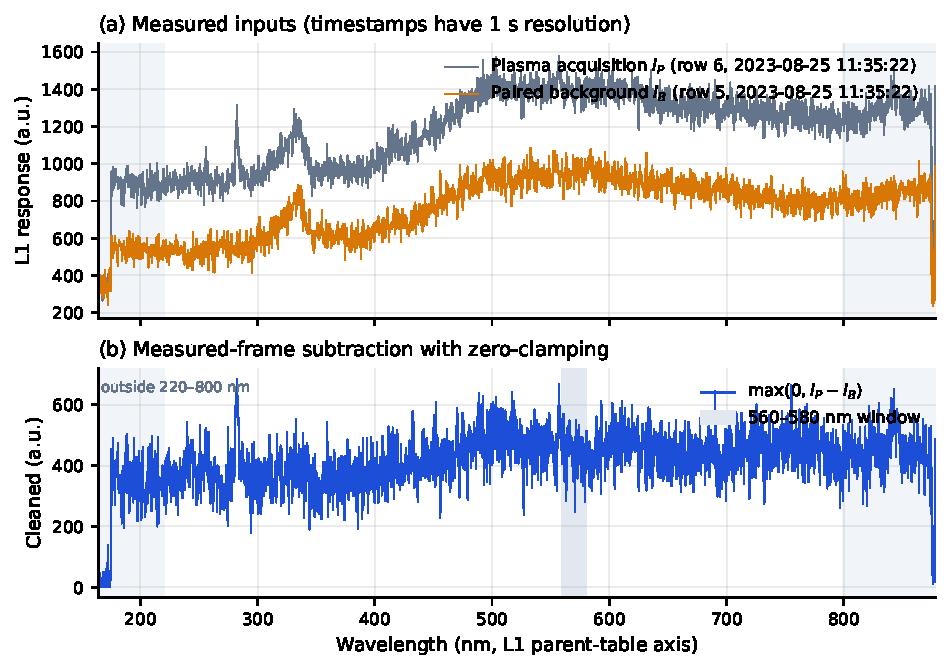
\includegraphics[width=0.75\textwidth]{../figures/fig3_background_subtraction}
    \caption{Measured-frame subtraction for Measurement ID~3 over the full stored range (shaded: outside 220--800~nm). (a) Plasma acquisition $I_P$ and the paired background $I_B$ from the preceding row; (b) $\max(0, I_P - I_B)$ with the 560--580~nm window used for $\sigma$. Wavelengths use the L1 parent-table axis.}
    \label{fig:bg_subtraction}
\end{figure*}

For ID~3 no residual is negative in 220--800~nm (0.48\% over all 2,094 channels); the clip fractions of IDs~1--4 are 22.5, 76.8, 0.5 and 28.1\%. Window statistics and the noise-propagation comparison, corrected for the unequal variances of $I_P$ and $I_B$, are descriptive and are given in Supplementary Section~S2 (Tables~S1--S2).

\textit{Clip fraction across the archive.} Of the 613 paired acquisitions, 372 (60.7\%), 256 (41.8\%) and 157 (25.6\%) exceed clip fractions of 0.25, 0.5 and 0.75 (Figure~\ref{fig:clip}); the distribution has modes near 0 and 1, so 0.5 is a convention, not a validated cut-off. Correlations with other signal measures are descriptive (Supplementary Section~S2). All acquisitions are stored; the clip fraction, paired-background row and subtraction flag are in \texttt{measurement\_clean} and the \texttt{\_params.csv} files, but no API endpoint returns them yet (\texttt{/api/v1/measurements}, \texttt{/api/v1/public/measurements}, \texttt{/api/v1/spectrum} and \texttt{/api/v1/public/spectra} were checked). The evaluations below exclude ID~2 (clip fraction 0.77).

\begin{figure*}[!t]
    \centering
    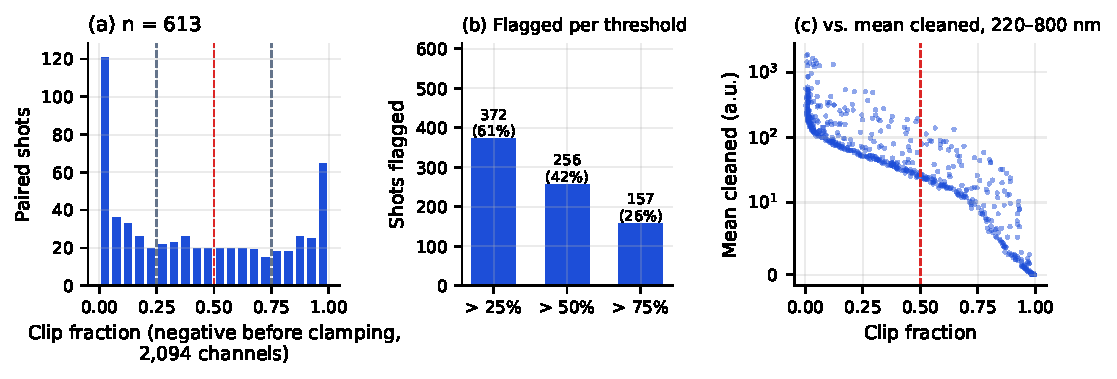
\includegraphics[width=\textwidth]{../figures/fig5_clipping}
    \caption{Clip fraction of the 613 paired acquisitions. (a) Distribution (dashed: 0.25/0.5/0.75); (b) acquisitions flagged per threshold; (c) clip fraction vs.\ mean cleaned intensity in 220--800~nm (descriptive).}
    \label{fig:clip}
\end{figure*}

\subsection{Downsampling}
\label{subsec:ds}

IDs 1, 3 and 4 were evaluated over the 1,684 calibrated-range channels (42, 59 and 73 detected peaks; $3\sigma=177.5$, 212.3 and 140.6~a.u.) and, separately, over all 2,094 channels (\texttt{revision\_v2/outputs/analysis/C\_downsampling.csv}). Table~\ref{table:downsampling} gives $k=4$ ($T=130$, i.e.\ 7.7\% of 1,684). RMSE is computed against the full-resolution spectrum after linear interpolation; retention counts detected peaks whose exact channel is in the output.

\begin{table}[!htbp]
\centering
\scriptsize
\setlength{\tabcolsep}{2pt}
\begin{tabular}{@{}lccc@{}}
\toprule
\textbf{Method (budget)} & \textbf{Points} & \textbf{Peaks (\%)} & \textbf{RMSE} \\
\midrule
\multicolumn{4}{@{}l}{\textit{Server (Python): 220--800~nm, 1,684 ch., $k=4$, $T=130$}} \\
Uniform ($T$) & 130 & 4.1--7.1 & 58.7--79.8 \\
Max-binning ($T$) & 130 & 86.3--94.9 & 111.2--125.5 \\
LTTB ($T$) & 130 & 45.8--59.5 & 71.1--93.6 \\
LTTB + 24-line list ($T$+24) & 150--151 & 47.5--61.9 & 69.3--91.2 \\
LTTB+Peaks ($T$+peaks) & 147--167 & 100 & 80.4--98.2 \\
LTTB, size of LTTB+Peaks & 147--167 & 50.8--57.1 & 66.6--88.8 \\
LTTB+Peaks, $\le T$ (eval.\ variant) & 129--130 & 100 & 85.6--105.2 \\
\midrule
\multicolumn{4}{@{}l}{\textit{Web viewer (TypeScript): 164--878~nm, 2,094 ch., $T=209$}} \\
LTTB ($T$) & 209 & 50.8--69.0 & 67.7--90.1 \\
LTTB + 32-line list ($T$+32) & 237--239 & 55.9--71.4 & 64.4--89.0 \\
\bottomrule
\end{tabular}
\caption{Downsampling of IDs 1, 3, 4 (ranges over IDs; per-ID values in \texttt{C\_downsampling.csv} and \texttt{C\_browser\_viewer.csv}). Upper block: server implementation, calibrated range. Peaks: detected peaks kept; RMSE in a.u. Lower block: the viewer's default configuration, run with the viewer's own code; RMSE over 2,094 channels, so not directly comparable with the upper block.}
\label{table:downsampling}
\end{table}

LTTB+Peaks keeps 100\% of detected peaks because they are its input, so its cost is the measurable quantity: it outputs 147--167 points instead of 130, and at an equal 130-point budget its RMSE exceeds that of LTTB by 9.0--22.0~a.u.\ (11.7--31.0\%). Reference wavelengths as targets preserve reference channels, not peaks: the server with the 24-line list keeps 47.5--61.9\% of peaks, and the viewer in its own configuration (TypeScript, run under Node.js) keeps 55.9--71.4\%, against 50.8--69.0\% for LTTB alone. The TypeScript and Python implementations returned identical channels in all 24 tested configurations. Uniform decimation has the lowest RMSE but discards most peaks, so no method is best on both measures; results for $k=1$--5 and both ranges are in Supplementary Section~S3.

\begin{figure*}[!t]
    \centering
    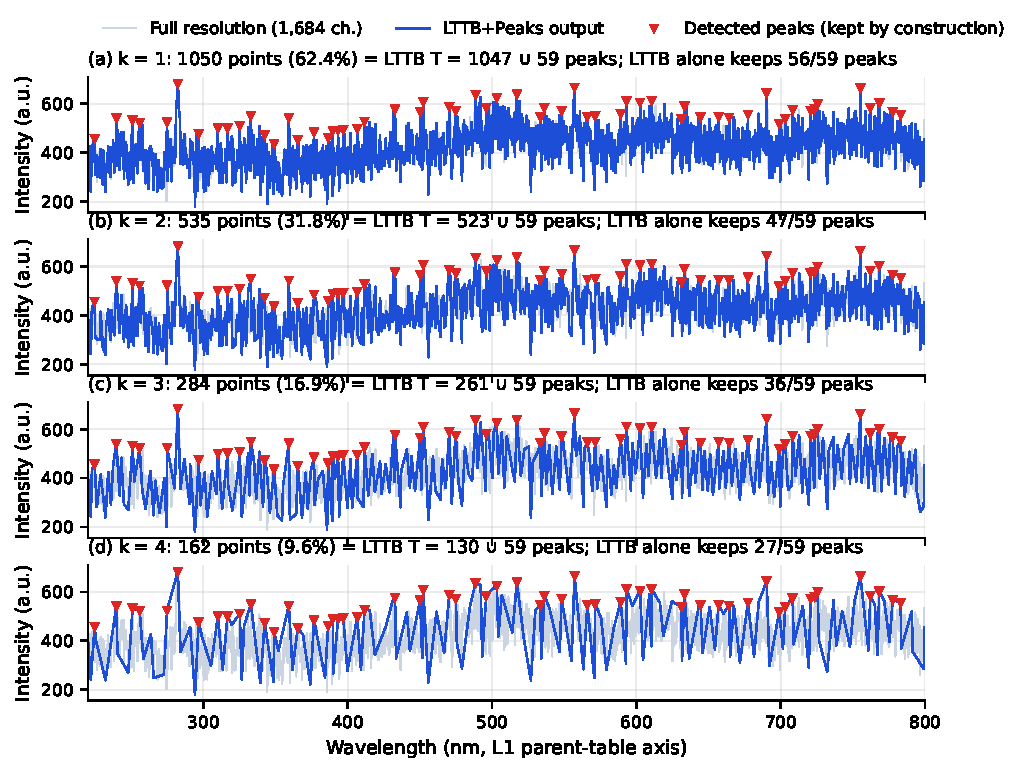
\includegraphics[width=0.8\textwidth]{../figures/fig2_downsampling}
    \caption{Server LTTB with the detected peaks of ID~3 as targets, $k=1$--4, calibrated range. Panel titles give the LTTB budget $T$, the resulting output size and the number of peaks LTTB alone would keep.}
    \label{fig:adaptive_zoom}
\end{figure*}

\subsection{Candidate annotation and a random-shift null model}

Table~\ref{table:elements} summarises IDs~1, 3 and 4; the per-peak table with signed offsets, prominences and all references within 0.5 and 1.1~nm is \texttt{D\_per\_line\_candidates.csv}. For ID~3 the eight coincidences lie near Fe~I, Ca~II, Mg~I, Na~I and O~I lines with offsets of $-0.09$ to $+0.48$~nm (Figure~\ref{fig:nist_annotated}); three have a second reference within 1.1~nm and cannot be assigned to one transition, and the labels do not imply that every listed species is present. The most prominent feature, at 282.3~nm, has no line of the 24-line reference list within 1.1~nm; the full NIST database was not searched. Near-misses are listed in Supplementary Section~S4.

\begin{figure*}[!t]
    \centering
    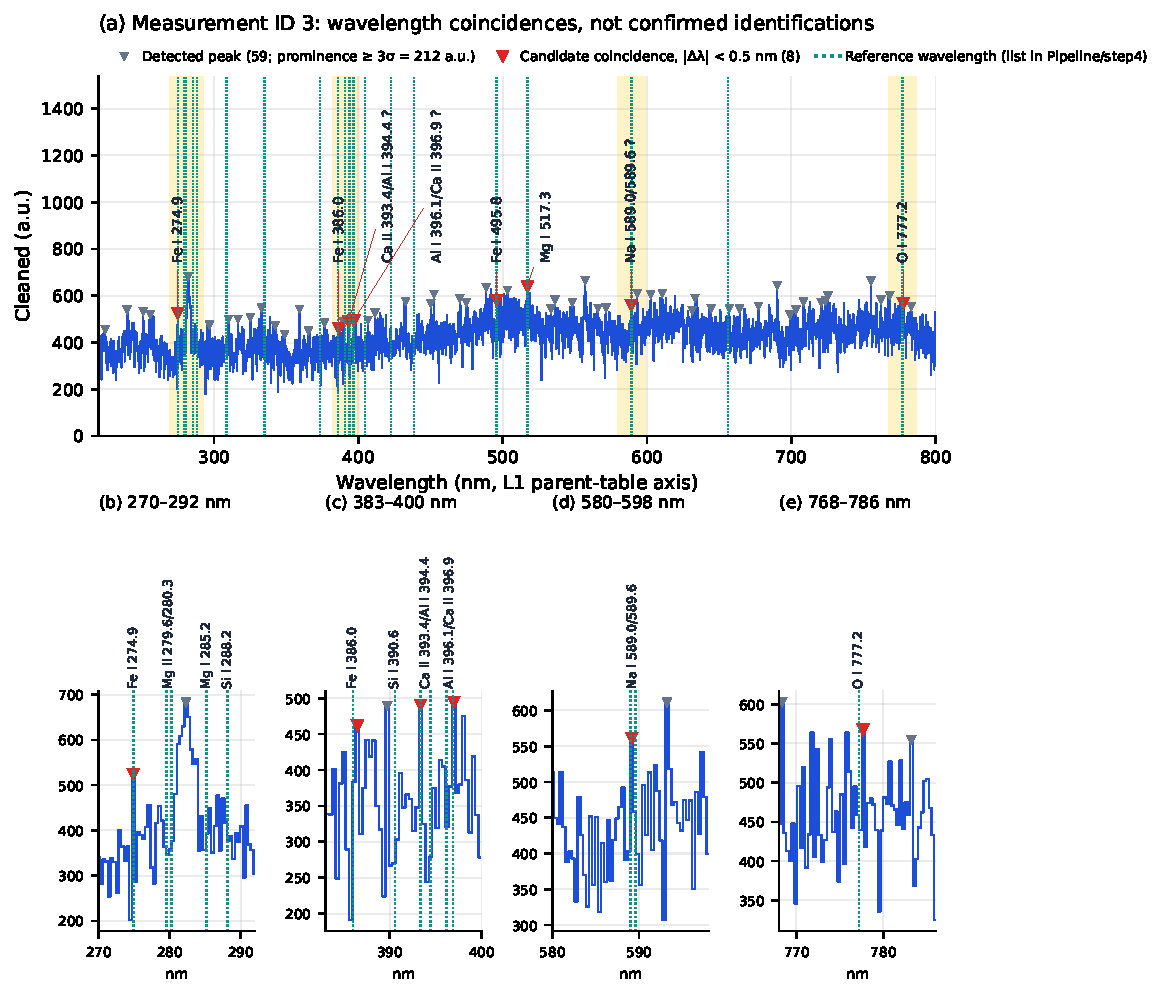
\includegraphics[width=\textwidth]{../figures/fig4_nist_annotated}
    \caption{Wavelength coincidences for Measurement ID~3 (not identifications). (a) Calibrated-range cleaned spectrum, detected peaks (grey), peaks with a reference within 0.5~nm (red; labels list all references within 1.1~nm, ``?'' where more than one), reference wavelengths (dotted). (b)--(e) Shaded windows at channel resolution; references closer than 1.1~nm share a label.}
    \label{fig:nist_annotated}
\end{figure*}

\textit{Null model.} Each draw shifts the whole 24-line list by one common offset, $|s|\sim U(2,20)$~nm with random sign, and re-applies the matching rule to the unchanged peaks; $p=(1+k)/(1+N)$ for $k$ of $N$ draws at or above the observed count. Single spectra use 10,000 draws. Archive-wide tests use 1,000 draws, each applying the same shift to every spectrum and summing the per-spectrum counts; the axis comparison uses the first 300 of them (Supplementary Section~S4).

\begin{table}[!htbp]
\centering
\scriptsize
\setlength{\tabcolsep}{2pt}
\begin{tabular}{@{}lrrrrrr@{}}
\toprule
\textbf{Spectra} & \textbf{Peaks} & \textbf{$N$} & \textbf{Obs.} & \textbf{Mean} & \textbf{$k$} & \textbf{$p$} \\
\midrule
ID 1 & 42 & 10,000 & 2 & 1.28 & 3,419 & 0.34 \\
ID 3 & 59 & 10,000 & 8 & 2.41 & 0 & 0.0001 \\
ID 4 & 73 & 10,000 & 5 & 2.31 & 617 & 0.062 \\
Archive (613) & 33,825 & 1,000 & 1,572 & 1,437.1 & 95 & 0.096 \\
Clip $\le0.5$ (357) & 21,678 & 1,000 & 959 & 863.9 & 79 & 0.080 \\
613, parent axis$^{a}$ & 33,825 & 300 & 1,572 & 1,440.0 & 30 & 0.10 \\
613, single-shot$^{a}$ & 33,825 & 300 & 1,386 & 1,451.8 & 215 & 0.72 \\
\bottomrule
\end{tabular}
\caption{Candidate coincidences ($|\Delta\lambda|<0.5$~nm, one per peak) and the random-shift null model (archive rows: sums over spectra): $N$ draws, observed count (Obs.), null mean, $k$ draws $\ge$ observed, $p=(1+k)/(1+N)$. $^{a}$Same detected channels labelled with either wavelength axis; first 300 archive draws.}
\label{table:elements}
\end{table}

Only ID~3 is statistically significantly enriched under the specified null ($p=0.0001$); IDs~1 and 4 and both archive-wide aggregates are not ($p\ge0.062$; Figure~\ref{fig:null}). With the single-shot wavelength axis the archive count falls below the null mean ($p=0.72$, against $p=0.10$ for the parent axis with the same draws). Enrichment, where present, concerns the peak and reference lists as a whole and does not validate any individual assignment. No line-ratio analysis is performed, because line ratios depend on plasma conditions, self-absorption and instrument response.

\begin{figure*}[!t]
    \centering
    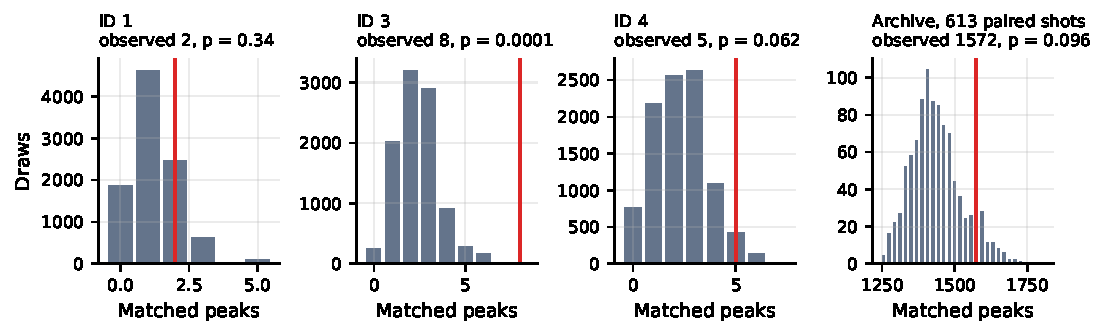
\includegraphics[width=\textwidth]{../figures/fig6_random_shift}
    \caption{Null distributions of coincidence counts under common random shifts of the reference list; red: observed.}
    \label{fig:null}
\end{figure*}

\subsection{API response performance}

\textit{Public deployment over the WAN.} On 23 October 2026 (22:32--23:28 IST) one client host sent 3,600 measured requests to \texttt{/api/v1/spectrum} of the public deployment in three sessions 15~min apart: two workloads, cache bypassed and warm, concurrency 1, 4 and 8, and 100 measured requests per setting after 10 warm-up requests. There were 0 errors and 0 timeouts (Table~\ref{table:wan}), and session medians agreed within 352~ms for full spectra and 105~ms for downsampled responses. With the cache bypassed the server reported about 530~ms of processing per request; the rest is network and transfer. Concurrency was capped at 8 to limit load on the shared deployment, so its saturation point was not determined.

\textit{Local loopback.} On one host with one server worker and the cache disabled, full spectra took a median 19.9~ms at concurrency 1 and 717.7~ms at 32 (41.7--45.2 requests/s, limited by the single worker), and 130-point responses 8.6 and 230.9~ms (14,400 requests, 0 errors). On a freshly loaded database without planner statistics the spectrum query ran as a nested-loop join (422~ms instead of about 1~ms), so ingestion now ends with \texttt{ANALYZE}. Protocols, the local table and the earlier single-session July 2026 campaign are in Supplementary Section~S5.

\begin{table}[!htbp]
\centering
\scriptsize
\setlength{\tabcolsep}{2.5pt}
\begin{tabular}{@{}llrrrrr@{}}
\toprule
\textbf{Workload} & \textbf{Cache} & \textbf{Conc.} & \textbf{P50} & \textbf{P95} & \textbf{P99} & \textbf{Req/s} \\
\midrule
2,094 pts & bypassed & 1 & 1,049.6 & 1,406.3 & 1,581.9 & 1.0 \\
             &          & 4 & 1,173.7 & 1,654.3 & 1,790.6 & 3.3 \\
             &          & 8 & 1,850.1 & 2,561.2 & 2,753.5 & 4.2 \\
             & warm     & 1 & 402.4   & 957.9   & 1,109.6 & 2.1 \\
             &          & 4 & 575.3   & 1,125.7 & 1,349.9 & 6.2 \\
             &          & 8 & 1,147.2 & 1,665.6 & 1,811.3 & 6.8 \\
LTTB $k{=}4$, 130 pts & bypassed & 1 & 787.7 & 907.3   & 1,050.4 & 1.3 \\
             &          & 4 & 656.4   & 1,090.0 & 1,322.1 & 5.4 \\
             &          & 8 & 785.3   & 1,229.3 & 1,395.2 & 9.2 \\
             & warm     & 1 & 264.7   & 323.3   & 560.8   & 3.5 \\
             &          & 4 & 272.9   & 305.4   & 822.0   & 13.5 \\
             &          & 8 & 267.9   & 321.7   & 407.6   & 26.6 \\
\bottomrule
\end{tabular}
\caption{Public deployment over the WAN: latency (ms) and throughput, medians over three sessions (per-session values and raw latencies in \texttt{revision\_v2/outputs/benchmark\_wan/}).}
\label{table:wan}
\end{table}

\section{Conclusions}

LunarAtlas converts the Chandrayaan-3 LIBS L1 archive into relational, L1-derived records with recorded provenance. On the full 301-product archive copy every data file matched its label checksum, and 613 of 745 plasma acquisitions were paired and stored as cleaned. Processing is deterministic, re-ingestion is idempotent, and every stored cleaned value equals the subtraction recomputed from the stored raw values. The downsampler can preserve any caller-specified channels at a quantified RMSE cost. The software does not identify elements: wavelength coincidences with a short reference list are statistically significantly enriched under the specified null in one of three worked-example spectra and not archive-wide, and the archive itself carries two wavelength scales that differ by about 5--11~nm.

\paragraph{Limitations} Detailed spectral metrics come from one product. The clip-fraction threshold is a convention. The L1 wavelength scale is ambiguous and not corrected. Background stability cannot be checked below the 1~s timestamp resolution, and some pairs span 13~s. WAN latency was measured from one client location on one evening at concurrency up to 8, so the deployment's saturation point is unknown. The demonstration deployment still holds legacy records, and the stored quality fields are not yet returned by the API. No Level-2 (abundance) calibration is implemented. Details of all evaluations are in the supplementary material.

\paragraph{Future work} Resolving the archive wavelength-scale question with the data providers; plasma-diagnostic, line-ratio and abundance analyses built on the provided L1-derived records; and WAN measurements from several client locations and at higher concurrency on a non-shared deployment.

\section*{Author Contributions}
\textbf{Lovekesh Anand:} Conceptualisation, Investigation, Methodology, Software, Validation, Formal Analysis, Data Curation, Writing -- Original Draft, Visualisation.

\textbf{Dua Saeed:} Investigation, Software, Validation, Formal Analysis, Data Curation, Writing -- Original Draft

\section*{Declaration of Competing Interests}
The authors declare no known competing financial interests or personal relationships that could have influenced the work reported in this paper.

\section*{Funding}
This research received no specific grant from funding agencies in the public, commercial, or not-for-profit sectors.

\section*{Acknowledgements}
The authors thank ISRO for making the Chandrayaan-3 LIBS Level-1 data public through PRADAN. Reference wavelengths were taken from the NIST Atomic Spectra Database.

\section*{Software Availability}
\begin{itemize}
    \item \textbf{Authors:} Lovekesh Anand, Dua Saeed --- Maharshi Dayanand University, Rohtak, Haryana, India
    \item \textbf{Repository:} \url{https://github.com/LovekeshAnand/LunarAtlas} \quad \textbf{License:} MIT
    \item \textbf{Archived version:} \url{https://doi.org/10.5281/zenodo.20771542} (v1.0.1; does not yet contain the revision changes) \cite{lunaratlas_zenodo}
    \item \textbf{Reproduction of this paper's numbers:} \texttt{revision\_v2/} (audit, processing, ingestion, analysis, figures, benchmark scripts and their outputs)
    \item \textbf{Supplementary material:} \texttt{revision\_v2/paper/supplementary.pdf} (Sections S1--S5, Tables S1--S3)
\end{itemize}

\section*{Data Availability}
The Chandrayaan-3 LIBS Level-1 data are available from PRADAN at \url{https://pradan.issdc.gov.in}. This work used a local copy of collection \texttt{lib-v2} (labels created 2024-05-16); the date on which it was originally downloaded was not recorded. The input-file manifest with label and computed checksums is \path{revision_v2/outputs/archive_audit/input_manifest.csv}.

\section*{Declaration of Generative AI and AI-assisted Technologies}
During the preparation of this work, the authors used ChatGPT (OpenAI) and Claude (Anthropic) to improve readability and language. Claude was also used to draft revised manuscript text and the response to reviewers, to review code, and to write and run the audit, analysis, figure, benchmark and migration-rehearsal scripts in \texttt{revision\_v2/} and the corresponding pipeline and ingestion changes. The authors reviewed and edited the content as needed and take full responsibility for the content of the publication.

\renewcommand{\bibfont}{\scriptsize}
\setlength{\bibsep}{0pt}
\bibliographystyle{elsarticle-num}
\bibliography{paper}

\end{document}
